\documentclass{amsart}

\usepackage[utf8]{inputenc}
\usepackage[T2A]{fontenc}
\usepackage[english,russian]{babel}
\usepackage{amsthm,amsmath,amsfonts,amssymb}
\usepackage{fullpage}
\usepackage{eufrak}
\usepackage{bbm}

%%% Дополнительная работа с математикой
\usepackage{amsfonts,amssymb,amsthm,mathtools} % AMS
\usepackage{amsmath}
\usepackage{icomma}

%% Шрифты
\usepackage{euscript}	% Шрифт Евклид
\usepackage{mathrsfs}	% Красивый матшрифт

%% Свои команды
\DeclareMathOperator{\lb}{\mathop{lb}}	% логарифм по основанию 2
\DeclareMathOperator{\sgn}{\mathop{sgn}}	% сигнум
\renewcommand{\Im}{\mathop{\mathrm{Im}}\nolimits}	% мнимая часть
\renewcommand{\Re}{\mathop{\mathrm{Re}}\nolimits}	% вещественная часть
\renewcommand{\emptyset}{\varnothing}	% пустое множество
\renewcommand{\le}{\leqslant}	% отечественная версия "меньше или равно"
\renewcommand{\ge}{\geqslant}	% отечественная версия "больше или равно"
\renewcommand{\epsilon}{\varepsilon}	% стандартная "эпсилон"
\renewcommand{\phi}{\varphi}	% стандартная "фи"
\newcommand{\const}{\mathrm{const}}	% константа

%% Множества чисел
\DeclareMathOperator{\Natural}{\mathbb{N}}	% Натуральные числа
\DeclareMathOperator{\Integer}{\mathbb{Z}}	% Целые числа
\DeclareMathOperator{\Integerp}{\mathbb{Z}_{+}}	% Целые неотрицательные числа
\DeclareMathOperator{\Rational}{\mathbb{Q}}	% Рациональные числа
\DeclareMathOperator{\Real}{\mathbb{R}}	% Вещественные числа
\DeclareMathOperator{\Realp}{\mathbb{R}_{>0}}	% Вещественные положительные числа
\DeclareMathOperator{\Realn}{\mathbb{R}_{<0}}	% Вещественные отрицательные числа
\DeclareMathOperator{\Realnn}{\mathbb{R}_{\ge 0}}	% Вещественные неотрицательные числа
\DeclareMathOperator{\Realnp}{\mathbb{R}_{\le 0}}	% Вещественные неположительные числа
\DeclareMathOperator{\Complex}{\mathbb{C}}	% Комплексные числа

%% Заглавные греческие буквы
\DeclareMathOperator{\Alpha}{\mathrm{A}}	% Альфа
\DeclareMathOperator{\Beta}{\mathrm{B}}	% Вета
\DeclareMathOperator{\Epsilon}{\mathrm{E}}	% Эпсилон
\DeclareMathOperator{\Zeta}{\mathrm{Z}}	% Дзета
\DeclareMathOperator{\Eta}{\mathrm{H}}	% Эта
\DeclareMathOperator{\Iota}{\mathrm{I}}	% Йота
\DeclareMathOperator{\Kappa}{\mathrm{K}}	% Каппа
\DeclareMathOperator{\Mu}{\mathrm{M}}	% Мю
\DeclareMathOperator{\Nu}{\mathrm{N}}	% Ню
\DeclareMathOperator{\Omicron}{\mathrm{O}}	% Омикрон
\DeclareMathOperator{\Rho}{\mathrm{P}}	% Ро
\DeclareMathOperator{\Tau}{\mathrm{T}}	% Тау
\DeclareMathOperator{\Chi}{\mathrm{X}}	% Хи

%% Теория вероятностей
\renewcommand{\Prob}{\mathbb P}	% вероятность
\newcommand{\Expect}{\mathbb E}	% математическое ожидание
\renewcommand{\Variance}{\mathbb D}	% дисперсия
\newcommand{\Entropy}{\mathbb H}	% энтропия
\DeclareMathOperator{\cov}{\mathop{cov}}	% ковариация
\DeclareMathOperator{\supp}{\mathop{supp}}	% носитель
\DeclareMathOperator{\Skewness}{\mathop{Skew}}	% коэффициент асимметрии
\DeclareMathOperator{\Kurtosis}{\mathop{Kurt}}	% коэффициент эксцесса

%%% Статистический анализ
\newcommand*{\moment}[1]{\overline{#1}}	% выборочный момент
\DeclareMathOperator{\hskew}{\mathop{\widehat{Skew}}}	% выборочный коэффициент асимметрии
\DeclareMathOperator{\hkurt}{\mathop{\widehat{Kurt}}}	% выборочный коэффициент эксцесса
%% Однопараметрические распределения
\newcommand*{\chisq}[1]{\chi^2_{#1}}	% Распределение хи-квадрат
\newcommand*{\Stud}[1]{\mathcal{S}_{#1}}	% Распределение Стьюдента
\newcommand*{\Exp}[1]{\mathop{\mathrm{Exp}}(#1)}	% Показательное распределение
\newcommand*{\Bern}[1]{\mathop{\mathrm{Bern}}(#1)}	% Распределение Бернулли
\newcommand*{\Geom}[1]{\mathop{\mathrm{Geom}}(#1)}	% Геометрическое распределение
\newcommand*{\Pois}[1]{\mathop{\mathrm{Pois}}(#1)}	% Распределение Пуассона
%% Двухпараметрические распределения
\newcommand*{\FS}[2]{\mathcal{F}_{#1, #2}}	% Распределение Фишера-Снедекора
\newcommand*{\Norm}[2]{\mathcal{N}(#1, #2)}	% Нормальное распределение
\newcommand*{\Unif}[2]{\mathcal{U}(#1, #2)}	% Равномерное распределение
\newcommand*{\DE}[2]{\mathop{\mathrm{DE}}(#1, #2)}	% Распределение Лапласа
\newcommand*{\Cauchy}[2]{\mathop{\mathrm{C}}(#1, #2)}	% Распределение Коши
\newcommand*{\Binom}[2]{\mathop{\mathrm{Binom}}(#1, #2)}	% Биномиальное распределение
\newcommand*{\Betadist}[2]{\mathop{\mathrm{Beta}}(#1, #2)}	% Бета-распределение
\newcommand*{\Gammadist}[2]{\mathop{\mathrm{Gamma}}(#1, #2)}	% Гамма-распределение
%% Ажурные и готические буквы
\newcommand*{\Acl}{\mathcal{A}}	% A красивое
\newcommand*{\Ccl}{\mathcal{C}}	% C красивое
\newcommand*{\Fcl}{\mathcal{F}}	% F красивое
\newcommand*{\Icl}{\mathcal{I}}	% I красивое
\newcommand*{\Kcl}{\mathcal{K}}	% K красивое
\newcommand*{\Pcl}{\mathcal{P}}	% P красивое
\newcommand*{\Ycl}{\mathcal{Y}}	% Y красивое
\newcommand*{\Afr}{\mathfrak{A}}	% A готическое
\newcommand*{\Bfr}{\mathfrak{B}}	% B готическое
\newcommand*{\Ffr}{\mathfrak{F}}	% F готическое
\newcommand*{\Kfr}{\mathfrak{K}}	% K готическое
\newcommand*{\Xfr}{\mathfrak{X}}	% X готическое
%% Теория оценивания
\newcommand*{\ind}[1]{\mathbbm{1}_{\lbrace #1 \rbrace}}	% индикаторная функция
\newcommand*{\bias}[2]{\mathop{\mathrm{bias}}\nolimits_{#1}(#2)}	% смещение

%% Перенос знаков в формулах (по Львовскому)
\newcommand*{\hm}[1]{#1\nobreak\discretionary{}
	{\hbox{$\mathsurround=0pt #1$}}{}}

%%% Работа с картинками
\usepackage{graphicx,xcolor}	% Для вставки рисунков
\graphicspath{{images/}{images2/}}	% папки с картинками
\setlength\fboxsep{3pt}	% Отступ рамки \fbox{} от рисунка
\setlength\fboxrule{1pt}	% Толщина линий рамки \fbox{}
\usepackage{wrapfig}	% Обтекание рисунков и таблиц текстом
\RequirePackage{caption}
\DeclareCaptionLabelSeparator{defffis}{ "--- }
\captionsetup{justification=centering,labelsep=defffis}
\usepackage{float}
\usepackage{tikz}
\usepackage{pgfplots}
\pgfplotsset{compat=newest}
\usetikzlibrary{patterns}
\usetikzlibrary{calc}

%%% Работа с таблицами
\usepackage{array,tabularx,tabulary,booktabs}	% Дополнительная работа с таблицами
\usepackage{longtable}	% Длинные таблицы
\usepackage{multirow}	% Слияние строк в таблице
\usepackage{makecell}
\usepackage{multicol}


\renewcommand{\qedsymbol}{}

\newtheorem{problem}{Задание}

\begin{document}
	\newcommand{\problemset}[1]{
		\begin{center}
			\Large #1
		\end{center}
	}

	\begin{tabbing}
	\hspace{11cm} \= Студент: \= Божко-Домбровский Тимофей \\																			
	\> Группа: \> 2375 \\
	\> Вариант: \> 5 \\	
	\> Дата: \> \today
\end{tabbing}
\hrule
\vspace{1cm}	% файл с заголовком
	\problemset{Теория вероятностей и математическая статистика}
\problemset{Индивидуальное домашнее задание №3}

% Команда ниже задает "название" или слово, которое будет
% отображаться вместо proof или "доказательство"
% поскольку у нас в ИДЗ задачи - то нужно слово "Решение"
\renewcommand*{\proofname}{Решение}

Случайный вектор $(\xi,\eta)$ имеет равномерное распределение в области $D$:
\[
D = \{(x,y)\text{ }|\text{ }2x - y \ge 0, x \le 0, y \ge -2\}
\]
$\zeta = 3\xi^4 + 2$, $\nu = \lfloor 5\eta\rfloor$, $\mu = -4\xi + 2\eta$

%%%%%%%%%%%%%% ЗАДАНИЕ №1 %%%%%%%%%%%%%%
%% Условие задания №1
\begin{problem}
Найти $p_{\xi,\eta}(x,y)$, функции и плотности распределения компонент. Построить графики функций распределений $F_{\xi}(x)$ и $F_{\eta}(y)$. Будут ли компоненты независимыми?
\end{problem}

%% Решение задания №1
\begin{proof}
Случайный вектор имеет равномерное распределение в области D, значит что:
\[
p_{\xi,\eta}(x,y) = \begin{cases}
    C, & (x,y) \in D\\
    0, & \text{в отс. сл.}
    \end{cases}
\]
\begin{figure}[h!]
    \centering
    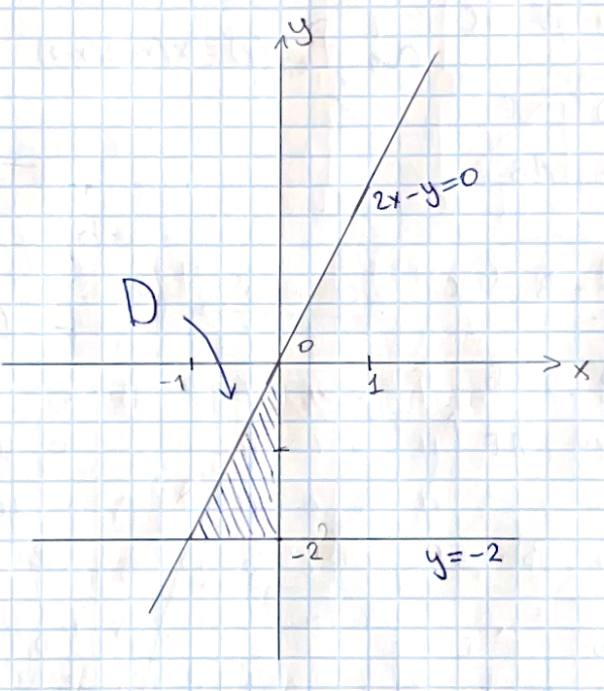
\includegraphics[width=0.5\linewidth]{1.jpeg}
    \caption{}
    \label{fig:enter-label}
\end{figure}
Изобразим область $D$ (см. рис. 1). По свойству имеем, что $ \iint_{\Real^2}p_{\xi,\eta}(x,y)dxdy = 1$:
\[
\iint_{\Real^2}p_{\xi,\eta}(x,y)dxdy = \iint_{D}p_{\xi,\eta}(x,y)dxdy = \int_{-1}^{0}dx\int_{-2}^{2x}Cdy = C = 1 \Rightarrow C = 1
\]
Итого:
\[
p_{\xi,\eta}(x,y) = \begin{cases}
    1, & (x,y) \in D\\
    0, & \text{в отс. сл.}
    \end{cases}
\]
Найдем плотности распределения компонент.\\
Для компоненты $\xi$:
\begin{gather*}
\int_{\Real}p_{\xi,\eta}(x,y)dy = \int_{-2}^{2x}dy = 2x + 2\\
p_{\xi}(x) = \begin{cases}
    2x + 2, & x \in [-1;0]\\
    0, & \text{в отс. сл.}
    \end{cases}
\end{gather*}
Для компоненты $\eta$:
\begin{gather*}
\int_{\Real}p_{\xi,\eta}(x,y)dx = \int_{y/2}^{0}dx = -\frac{y}{2}\\
p_{\eta}(x) = \begin{cases}
    -\frac{y}{2}, & y \in [-2;0]\\
    0, & \text{в отс. сл.}
    \end{cases}
\end{gather*}
Проверим компоненты на независимость. Должно выполняться условие $p_{\xi,\eta}(x,y) = p_{\xi}(x)\cdot p_{\eta}(y)$ во всех точках.
\[
1 = -\frac{y}{2}\cdot(2x + 2)\\
\]
Рассмотрим точку (0,0):
\[
1 = -\frac{0}{2}\cdot(2\cdot 0 + 2) = 0 - \text{неверно}\Rightarrow\text{компоненты зависимы}
\]
Найдем функции распределений$F_{\xi}(x)$ и $F_{\eta}(y)$ и построим их графики.
\[
F_{\xi}(x) = \int\limits_{-\infty}^{x}p_{\xi}(t)dt = \begin{cases}
    0, & x\in (-\infty;-1]\\
    (x + 1)^2, & x\in (-1; 0]\\
    1, & x\in (0;\infty)
\end{cases}
\]
\[
F_{\eta}(y) = \int\limits_{-\infty}^{y}p_{\eta}(t)dt = \begin{cases}
    0, & y\in (-\infty;-2]\\
    -\frac{y}{4} + 1, & y\in (-2; 0]\\
    1, & y\in (0;\infty)
\end{cases}
\]
Их графики на рисунке 2 соответственно.
\begin{figure}[h!]
    \centering
    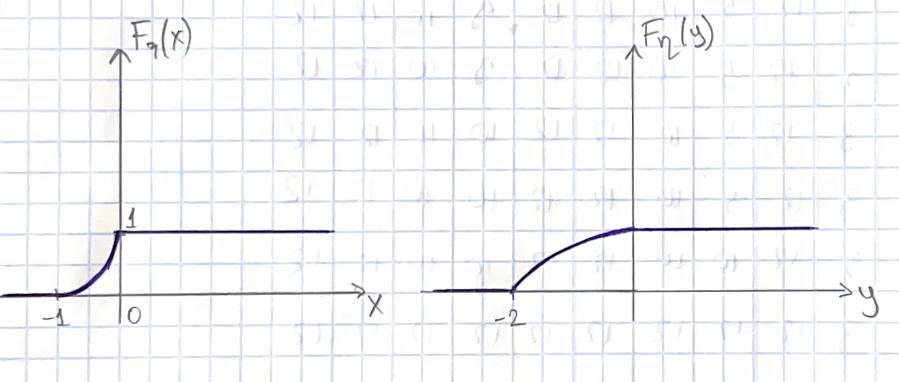
\includegraphics[width=0.5\linewidth]{2.jpeg}
    \caption{}
    \label{fig:enter-label}
\end{figure}
\end{proof}

%%%%%%%%%%%%%% ЗАДАНИЕ №2 %%%%%%%%%%%%%%
%% Условие задания №2
\begin{problem}
Найти распределения случайных величин $\zeta$ и $\nu$. Вычислить $\Expect\zeta$, $\Variance\zeta$, $\Expect\nu$ и $\Variance\nu$. Построить графики функций распределений $F_{\zeta}(z)$ и $F_{\nu}(n)$.
\end{problem}

%% Решение задания №2
\begin{proof}
$\zeta = 3\xi^4 + 2$. $\supp\xi = [-1;0]$, $\supp\zeta = [2;5]$. $g(\xi) = 3\xi^4 + 2$ и $g(\xi)$ монотонно убывает на $\supp\xi$. Тогда:
\begin{gather*}
g^{-1}(z) = -\sqrt[4]{\frac{z - 2}{3}}\\
(g^{-1}(z))' = \frac{-1}{4\sqrt[4]{3(z - 2)^3}}\\
\end{gather*}
Итого:
\[
p_{\zeta}(z) = \begin{cases}
    \frac{1}{2\sqrt[4]{3(z - 2)^3}}\cdot\left(1 - \sqrt[4]{\frac{z - 2}{3}}\right), & z \in [2;5]\\
    0, & \text{в отс. сл.}
    \end{cases}
\]
Считаем мат.ожидание и дисперсию:
\begin{gather*}
    \Expect\zeta = \int_{-\infty}^{\infty}z\cdot p_{\zeta}(z)dz = \int_{2}^{5}z\cdot p_{\zeta}(z)dz = \frac{11}{5} = 2.2\\
    \Expect\zeta^2 = \int_{-\infty}^{\infty}z^2\cdot p_{\zeta}(z)dz = \int_{2}^{5}z^2\cdot p_{\zeta}(z)dz = 5\\
    \Variance\zeta = \Expect\zeta^2 - \left(\Expect\zeta\right)^2 = 5 - 4.84 = 0.16
\end{gather*}
Функция распределения (график на рис. 3):
\[
F_{\zeta}(z) = \int\limits_{-\infty}^{z}p_{\zeta}(t)dt = \begin{cases}
    0, & z\in (-\infty;2]\\
    2\sqrt[4]{\frac{z - 2}{3}} - \sqrt{\frac{z - 2}{3}}, & z\in (2; 5]\\
    1, & z\in (5;\infty)
\end{cases}
\]
\begin{figure}[h!]
    \centering
    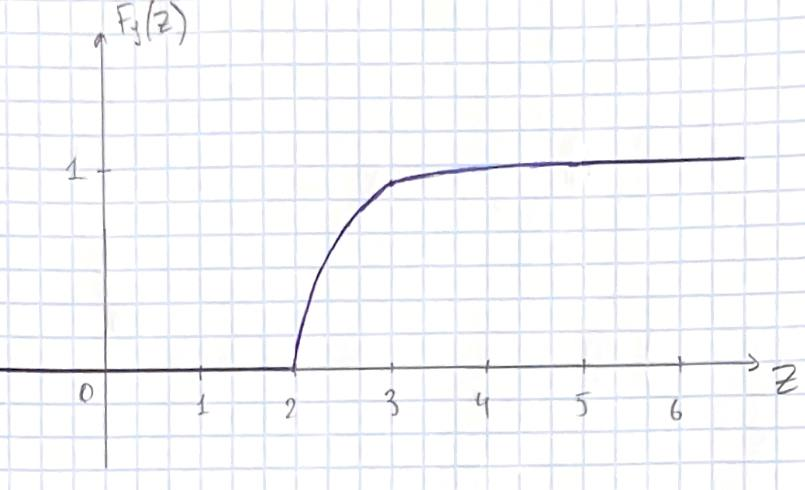
\includegraphics[width=0.5\linewidth]{3.jpeg}
    \caption{}
    \label{fig:enter-label}
\end{figure}
$\nu = \lfloor5\eta\rfloor$. $\supp\eta = [-2;0]$, $\supp\nu = \{-10, -9, -8, -7, -6, -5, -4, -3, -2, -1, 0\}$.
\[
\Prob(\nu = k) = \Prob(\eta\in[k/5; (k + 1)/5)) = -\int_{\frac{k}{5}}^{\frac{k + 1}{5}}\frac{y}{2}dy = \frac{-2k + 1}{100}
\]
Помимо этого учитываем, что для $\nu = 0$ $\eta = 0$, а значит $\Prob(\nu = 0) = 0$.\\
Строим таблицу:\\
\begin{table}[h!]
    \centering
    \begin{tabular}{|c|c|c|c|c|c|c|c|c|c|c|c|c|}
    \hline
        $\nu$ & -10 & -9 & -8 & -7 & -6 & -5 & -4 & -3 & -2 & -1 & 0 & $\sum$\\
    \hline
        $p_i$ & 0.19 & 0.17 & 0.15 & 0.13 & 0.11 & 0.09 & 0.07 & 0.05 & 0.03 & 0.01 & 0 & 1\\
    \hline
    \end{tabular}
\end{table}

Теперь считаем мат.ожидание и дисперсию:
\begin{gather*}
    \Expect\nu = \sum_{i: p_i > 0}a_ip_i = -7.15\\
    \Expect\nu^2 = \sum_{i: p_i > 0}a_i^2p_i = 56.65\\
    \Variance\nu = \Expect\nu^2 - \left(\Expect\nu\right)^2 = 56.65 - 51.1225 = 5.5275
\end{gather*}
Функция распределения (график на рис. 4):
\[
F_{\nu}(n) = \begin{cases}
    0, & n\in (-\infty;-10]\\
    0.19, & n\in (-10;-9]\\
    0.36, & n\in (-9;-8]\\
    0.51, & n\in (-8;-7]\\
    0.64, & n\in (-7;-6]\\
    0.75, & n\in (-6;-5]\\
    0.84, & n\in (-5;-4]\\
    0.91, & n\in (-4;-3]\\
    0.96, & n\in (-3;-2]\\
    0.99, & n\in (-2;-1]\\
    1, & n\in (-1;\infty)
\end{cases}
\]
\begin{figure}[h!]
    \centering
    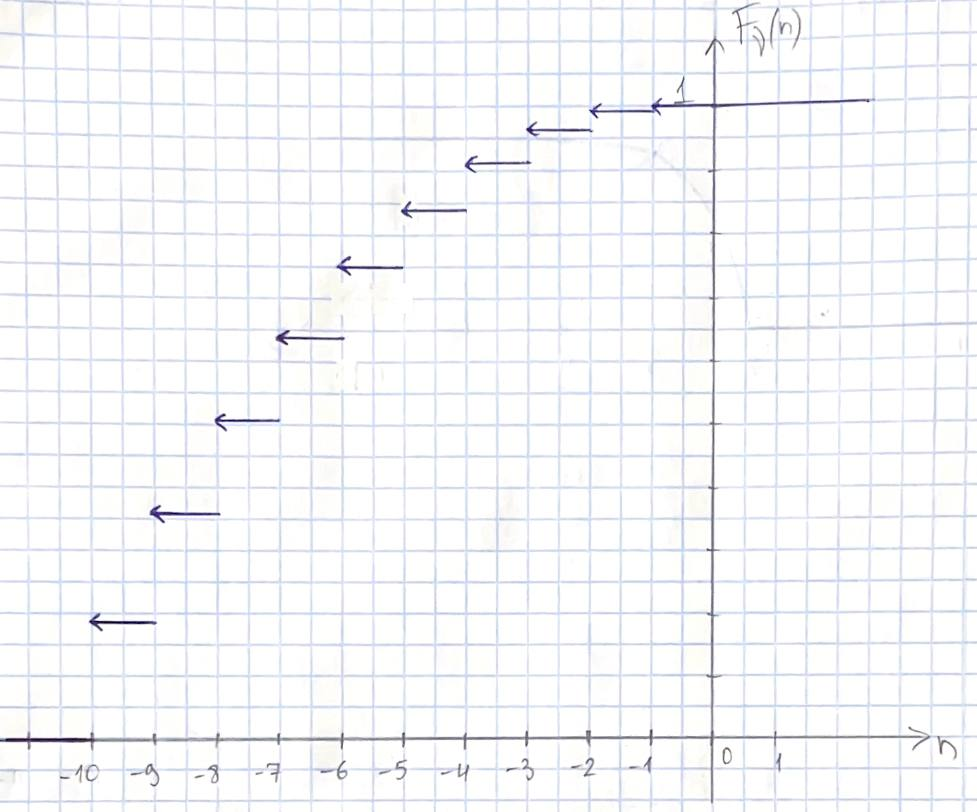
\includegraphics[width=0.5\linewidth]{4.jpeg}
    \caption{}
    \label{fig:enter-label}
\end{figure}
\end{proof}

%%%%%%%%%%%%%% ЗАДАНИЕ №3 %%%%%%%%%%%%%%
%% Условие задания №3
\begin{problem}
Вычислить вектор математических ожиданий, построить ковариационную и кореляционную матрицы для вектора $(\xi,\eta)$. Найти условное распределение $\xi$ при условии $\eta$. Вычислить $\Expect(\xi | \eta)$ и $\Variance(\xi | \eta)$.
\end{problem}

%% Решение задания №3
\begin{proof}
Мат.ожидание и дисперсия для $\xi$:
\begin{gather*}
    \Expect\xi = \int_{-\infty}^{\infty}x\cdot p_{\xi}(x)dx = \int_{-1}^{0}x\cdot(2x + 2)dx = -\frac{1}{3}\\
    \Expect\xi^2 = \int_{-\infty}^{\infty}x^2\cdot p_{\xi}(x)dx = \int_{-1}^{0}x^2\cdot(2x + 2)dx = \frac{1}{6}\\
    \Variance\xi = \Expect\xi^2 - \left(\Expect\xi\right)^2 = \frac{1}{6} - \frac{1}{9} = \frac{1}{18}
\end{gather*}
Мат.ожидание и дисперсия для $\eta$:
\begin{gather*}
    \Expect\eta = \int_{-\infty}^{\infty}y\cdot p_{\eta}(y)dy = \int_{-2}^{0}y\cdot\frac{-y}{2}dy = -\frac{4}{3}\\
    \Expect\eta^2 = \int_{-\infty}^{\infty}y^2\cdot p_{\eta}(y)dy = \int_{-2}^{0}y^2\cdot\frac{-y}{2}dy = 2\\
    \Variance\eta = \Expect\eta^2 - \left(\Expect\eta\right)^2 = 2 - \frac{16}{9} = \frac{2}{9}
\end{gather*}
Вектор мат.ожиданий:\\
\[
\Expect\begin{pmatrix} \xi \\ \eta \end{pmatrix} = \begin{pmatrix} -1/3 \\ -4/3 \end{pmatrix}
\]
Посчитаем ковариацию и корреляцию $\xi$ и $\eta$:
\begin{gather*}
\Expect\xi\eta = \iint_{\Real^2}xy\cdot p_{\xi,\eta}(x,y)dxdy = \int_{-1}^{0}dx\int_{-2}^{2x}xydy = \frac{1}{2}\\
\cov(\xi, \eta) = \Expect\xi\eta - \Expect\xi\cdot\Expect\eta = \frac{1}{2} = \frac{4}{9} = \frac{1}{18}\\
\rho(\xi,\eta) = \frac{\cov(\xi,\eta)}{\sqrt{\Variance\xi}\sqrt{\Variance\eta}} = \frac{1}{2}
\end{gather*}
Итого:
\[
\sum = \begin{pmatrix}
\frac{1}{18} & \frac{1}{18} \\
\frac{1}{18} & \frac{2}{9}
\end{pmatrix}
\]
\[
R = \begin{pmatrix}
1 & \frac{1}{2} \\
\frac{1}{2} & 1
\end{pmatrix}
\]
Найдем условное распределение $\xi$ при условии $\eta$:
\begin{gather*}
    p_{\xi|\eta=y_0} = \frac{p_{\xi,\eta}(x,y_0)}{p_{\eta}(y_0)} \text{ при } p_{\eta}(y) > 0\Rightarrow\\
    \Rightarrow p_{\xi|\eta=y_0} = \begin{cases}
        -\frac{2}{y_0}, & x\in [y_0/2; 0]\\
        0, & \text{в отс. сл.}
    \end{cases} \Rightarrow\\
    \Rightarrow p_{\xi|\eta} = \begin{cases}
        -\frac{2}{\eta}, & x\in [\eta/2; 0]\\
        0, & \text{в отс. сл.}
    \end{cases}
\end{gather*}
Условное мат.ожидание и условная дисперсия:
\begin{gather*}
    \Expect(\xi|\eta) = \int_{-\infty}^{\infty}x\cdot p_{\xi|\eta}(x)dx = \int_{\eta/2}^{0}x\cdot p_{\xi|\eta}(x)dx = \frac{\eta}{4}\\
    \Expect(\xi^2|\eta) = \int_{-\infty}^{\infty}x^2\cdot p_{\xi|\eta}(x)dx = \int_{\eta/2}^{0}x^2\cdot p_{\xi|\eta}(x)dx =\frac{\eta^2}{12}\\
    \Variance(\xi|\eta) = \Expect(\xi^2|\eta) - \left(\Expect(\xi|\eta)\right)^2 = \frac{\eta^2}{48}
\end{gather*}
Проверим свойство $\Expect(\Expect(\xi|\eta)) = \Expect\xi$:
\[
\Expect(\Expect(\xi|\eta)) = \Expect\left(\frac{\eta}{4}\right) = \frac{1}{4}\cdot\frac{-4}{3} = -\frac{1}{3} = \Expect\xi - \text{верно}
\]
Проверим свойство $\Expect(\Variance(\xi|\eta)) + \Variance(\Expect(\xi|\eta)) = \Variance\xi$:
\[
\Expect(\Variance(\xi|\eta)) + \Variance(\Expect(\xi|\eta)) = \Expect\left(\frac{\eta^2}{48}\right) + \Variance\left(\frac{\eta}{4}\right) = \frac{1}{24} + \frac{1}{72} = \frac{1}{18} = \Variance\xi - \text{верно}
\]
\end{proof}

%%%%%%%%%%%%%% ЗАДАНИЕ №4 %%%%%%%%%%%%%%
%% Условие задания №4
\begin{problem}
Найти распределение $\mu$. Вычислить $\Expect\mu$ и $\Variance\mu$. Построить график функции распределения $F_{\mu}(m)$.
\end{problem}

%% Решение задания №4
\begin{proof}
\begin{figure}[h!]
    \centering
    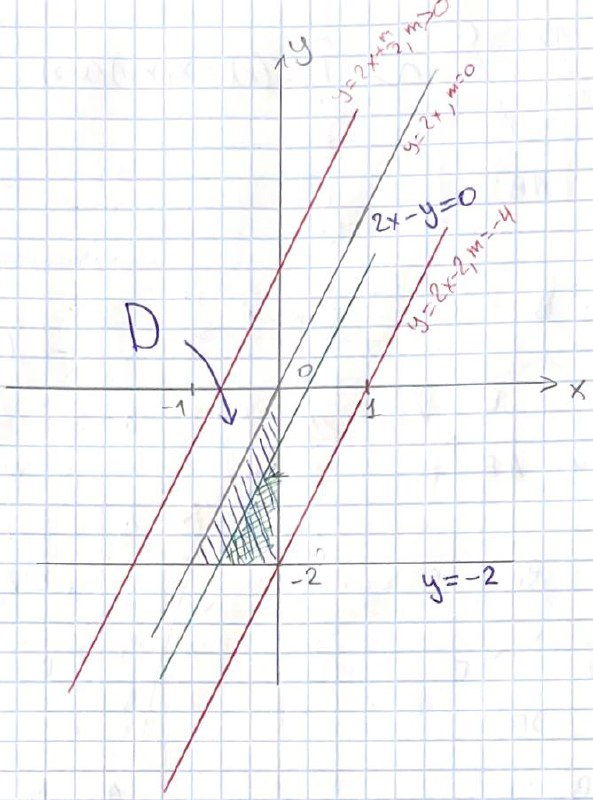
\includegraphics[width=0.5\linewidth]{5.jpeg}
    \caption{}
    \label{fig:enter-label}
\end{figure}
$\mu = -4\xi + 2\eta$. $F_{\mu}(m) = \Prob(\mu \le m) = \Prob(-4\xi + 2\eta\le m)$.\\
См. рис. 5. Из него слудует, что: 
\[
F_{\mu}(m) = \begin{cases}
    0, & m\in (-\infty;-4]\\
    \frac{(m + 4)^2}{16}& m\in (-4; 0]\\
    1, & m\in (0; \infty)
\end{cases}
\]
Зная функцию распределения находим плотность:
\[
p_{\mu}(m) = \begin{cases}
    \frac{m + 4}{8}& m\in [-4; 0]\\
    0, & \text{в отс. сл.}
\end{cases}
\]
Мат.ожидание и дисперсия:
\begin{gather*}
    \Expect\mu = \int_{-\infty}^{\infty}m\cdot p_{\mu}(m)dm = \int_{-4}^{0}m\cdot p_{\mu}(m)dm = -\frac{4}{3}\\
    \Expect\mu^2 = \int_{-\infty}^{\infty}m^2\cdot p_{\mu}(m)dm = \int_{-4}^{0}m^2\cdot p_{\mu}(m)dm = \frac{8}{3}\\
    \Variance\mu = \Expect\mu^2 - \left(\Expect\mu\right)^2 = \frac{8}{3} - \frac{16}{9} = \frac{8}{9}
\end{gather*}
График функции распределения на рисунке 6.
\begin{figure}[h!]
    \centering
    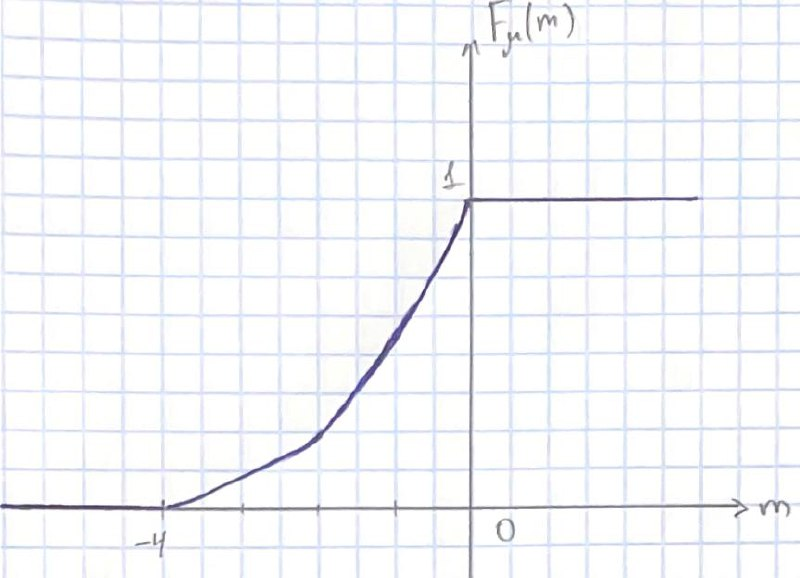
\includegraphics[width=0.5\linewidth]{6.jpeg}
    \caption{}
    \label{fig:enter-label}
\end{figure}
\end{proof}	% файл с решениями
        %\problemset{Теория вероятностей и математическая статистика}
\problemset{Индивидуальное домашнее задание №0}	% поменяйте номер ИДЗ

\renewcommand*{\proofname}{Решение}

%%%%%%%%%%%%%% ЗАДАНИЕ №1 %%%%%%%%%%%%%%
%% Условие задания №1
\begin{problem}
	Из урны, в которой лежат $ K $ белых и $ L $ чёрных шаров, наудачу выбирают один шар. Чему равна вероятность того, что этот шар "--- белый?
\end{problem}

%% Решение задания №1
\begin{proof}
	Пусть $ A $ "--- событие, что достали белый шар.
	Количество всех исходов будет равно: $ \#\Omega \hm= K + L $.
	
	Тогда количество благоприятных исходов (наступления события $ A $) равно: $ \#A = K $.
	
	Отсюда получаем, что вероятность наступления события $ A $ равна:
	\[ \Prob A = \cfrac{\#A}{\#\Omega} = \cfrac{K}{K + L}. \]
\end{proof}

%%%%%%%%%%%%%% ЗАДАНИЕ №2 %%%%%%%%%%%%%%
%% Условие задания №2
\begin{problem}
	Распределение случайной величины $ \xi $ задано таблицей:
	\begin{center}
		\begin{tabular}{|c|c|c|c|c|c|}
		\hline
		$ \xi $ & 1 & 2 & 4 & 6 & $ \Sigma $ \\
		\hline
		$ \mathbb{P} $ & 0,1 & 0,2 & 0,6 & 0,1 & 1 \\
		\hline
		\end{tabular}
	\end{center}
	Вычислить $ \Expect\xi $, $ \Variance\xi $, $ \Entropy\xi $ (в натах) и распределение $ \eta = \sin(\pi\xi/3) $.
\end{problem}

%% Решение задания №2
\begin{proof}
	Математическое ожидание дискретной случайной величины $ \xi $ задаётся формулой:
	\[ \Expect\xi = \sum_{i \colon p_i > 0}a_ip_i. \]
	Отсюда получаем:
	\[ \Expect\xi = 1 \cdot 0,1 + 2 \cdot 0,2 + 4 \cdot 0,6 + 6 \cdot 0,1 = 3,5. \]
	Дисперсия дискретной случайной величины $ \xi $ задаётся формулой:
	\[ \Variance\xi = \sum_{i \colon p_i > 0}(a_i - \mathbb E\xi)^2p_i. \]
	Отсюда получаем:
	\[ \Variance\xi = (1 - 3,5)^2 \cdot 0,1 + (2 - 3,5)^2 \cdot 0,2 + (4 - 3,5)^2 \cdot 0,6 + (6 - 3,5)^2 \cdot 0,1 = 1,85. \]
	Энтропия дискретной случайной величины $ \xi $ задаётся формулой:
	\[ \Entropy\xi = -\sum_{i \colon p_i > 0}p_i\log_bp_i. \]
	Необходимо вычислить энтропию в натах, т~е. $ b = e $. Получим:
	\[ \Entropy\xi = -(0,1 \cdot \ln0,1 + 0,2 \cdot \ln0,2 + 0,6 \cdot \ln0,6 + 0,1 \cdot \ln0,1) \approx 1,0889. \]
	Носитель случайной величины $ \xi $ имеет вид: $ \supp \xi = \lbrace 1, 2, 4, 6 \rbrace $. Тогда носитель случайной величины $ \eta $ будет иметь вид: $ \supp \eta = \left\lbrace -\frac{\sqrt{3}}{2}, 0, \frac{\sqrt{3}}{2} \right\rbrace  $. Найдём вероятности появления каждого числа:
	\begin{align*}
		\Prob(\eta = -\sqrt{3}/2) &= \Prob(\xi = 4) = 0,6. \\
		\Prob(\eta = 0) &= \Prob(\xi = 6) = 0,1. \\
		\Prob(\eta = \sqrt{3}/2) &= \Prob(\xi = 1) + \Prob(\xi = 2) = 0,3.
	\end{align*}
	Таким образом, можно записать распределение случайной величины $ \eta $ в виде таблицы:
	\begin{center}
		\begin{tabular}{|c|c|c|c|c|}
			\hline
			$ \eta $  & $ -\sqrt{3}/2 $ & 0   & $ \sqrt{3}/2 $ & $ \Sigma $ \\ \hline
			$ \Prob $ & 0,6             & 0,1 & 0,3            & 1          \\ \hline
		\end{tabular}
	\end{center}
\end{proof}

%%%%%%%%%%%%%% ЗАДАНИЕ №3 %%%%%%%%%%%%%%
%% Условие задания №3
\begin{problem}
	Условие задачи №3.
\end{problem}

%% Решение задания №3
\begin{proof}
	Решение задачи №3.
\end{proof}
\end{document}